% !TeX TXS-program:compile = txs:///pdflatex/[--shell-escape]
\documentclass[10pt,landscape,a4paper]{article}
\usepackage[table]{xcolor}
\usepackage[normalem]{ulem}
\usepackage{tikz}
\usetikzlibrary{shapes,positioning,arrows,fit,calc,graphs,graphs.standard}
\usepackage[nosf]{kpfonts}
\usepackage[t1]{sourcesanspro}
\usepackage{multicol}
\usepackage{wrapfig}
\usepackage[top=1mm,bottom=1mm,left=1mm,right=1mm]{geometry}
\usepackage[framemethod=tikz]{mdframed}
\usepackage{microtype}
\usepackage{tabularx}
\usepackage{hhline}
\usepackage{makecell}
\usepackage{mathtools}
\usepackage{subfig}
\usepackage{listings}
\usepackage{soul}
\usepackage{amsmath,amsthm,amsfonts,amssymb}

\graphicspath{ {./imgs/} }

\DeclarePairedDelimiter{\ceil}{\lceil}{\rceil}

\definecolor{myblue}{cmyk}{1,.72,0,.38}

\pgfdeclarelayer{background}
\pgfsetlayers{background,main}

\renewcommand{\baselinestretch}{.8}
\pagestyle{empty}

\let\counterwithout\relax
\let\counterwithin\relax
\usepackage{chngcntr}
\usepackage{verbatim}
\usepackage{etoolbox}
\makeatletter
\preto{\@verbatim}{\topsep=0pt \partopsep=0pt }
\makeatother

\counterwithin*{equation}{section}
\counterwithin*{equation}{subsection}
\usepackage{enumitem}
\newlist{legal}{enumerate}{10}
\setlist[legal]{label*=\arabic*.,leftmargin=3mm}
\setlist[itemize]{leftmargin=3mm}
\setlist[enumerate]{leftmargin=3.5mm}
\setlist{nosep}
\usepackage{minted}

\newenvironment{descitemize} % a mixture of description and itemize
{\begin{description}[leftmargin=*,before=\let\makelabel\descitemlabel]}
	{\end{description}}
\newcommand{\descitemlabel}[1]{%
	\textbullet\ \textbf{#1}%
}
\makeatletter

\renewcommand{\section}{\@startsection{section}{1}{0mm}%
	{.2ex}%
	{.2ex}%x
	{\color{myblue}\sffamily\small\bfseries}}
\renewcommand{\subsection}{\@startsection{subsection}{1}{0mm}%
	{.2ex}%
	{.2ex}%x
	{\sffamily\bfseries}}
\renewcommand{\subsubsection}{\@startsection{subsubsection}{1}{0mm}%
	{.2ex}%
	{.2ex}%x
	{\rmfamily\bfseries}}

\makeatother
\setlength{\parindent}{0pt}
\setminted{tabsize=2, breaklines}
% Remove belowskip of minted
\setlength\partopsep{-\topsep}

\newcolumntype{a}{>{\hsize=1.5\hsize}X}
\newcolumntype{b}{>{\hsize=.25\hsize}X}

\setlength\columnsep{10pt}
\setlength\columnseprule{0pt}
\begin{document}
	\abovedisplayskip=0pt
	\abovedisplayshortskip=0pt
	\belowdisplayskip=0pt
	\belowdisplayshortskip=0pt
	\scriptsize
%	\tiny
	\begin{multicols*}{4}
	\section{Constraint Satisfaction Problem}
	\begin{itemize}
		\item Aims to improve on systematic search as they tend to be computationally expensive by reducing search space
		\item Idea is to use factored representation of states (variables $X=\{x_1,\cdots,x_n\}$ where each has domain $D_i=\{d_1,\cdots,d_m\}$)
		\item If a state satisfies all constraint then it is a goal state
		\item CSPs systematically search for goal states by pruning invalid subtrees as early as possible
	\end{itemize}
	\subsection{CSP Formulation}
	\begin{itemize}
		\item State representation
		\begin{itemize}
			\item Variables: $X={x_1,...,x_n}$
			\item Domains: $D={d_1,...,d_k}$
			\item Initial state: All variables unassigned
			\item Intermediate state: Partial assignment
		\end{itemize}
		\item Goal Test: Each $c_i$ in constraints $C={c_1,...,c_m}$ are satisfied (Consistency) and all variables are assigned valid values (Complete)
		\item Actions: Assignment of values to variables (cost not used)
	\end{itemize}
	\subsection{Solving CSPs}
	\begin{itemize}
		\item We don't care about search path
		\item Use DFS to save space
		\item Backtracking algorithm: at each depth $l$: $(|X|-l\cdot|d|)$ states, total number of leaf states: $d^n$  (if order of variable not impt) else $n!m^n$, where $|X|$ = number of variable, $d$ is the domain and $m=|d|$
	\end{itemize}
	\begin{center}
		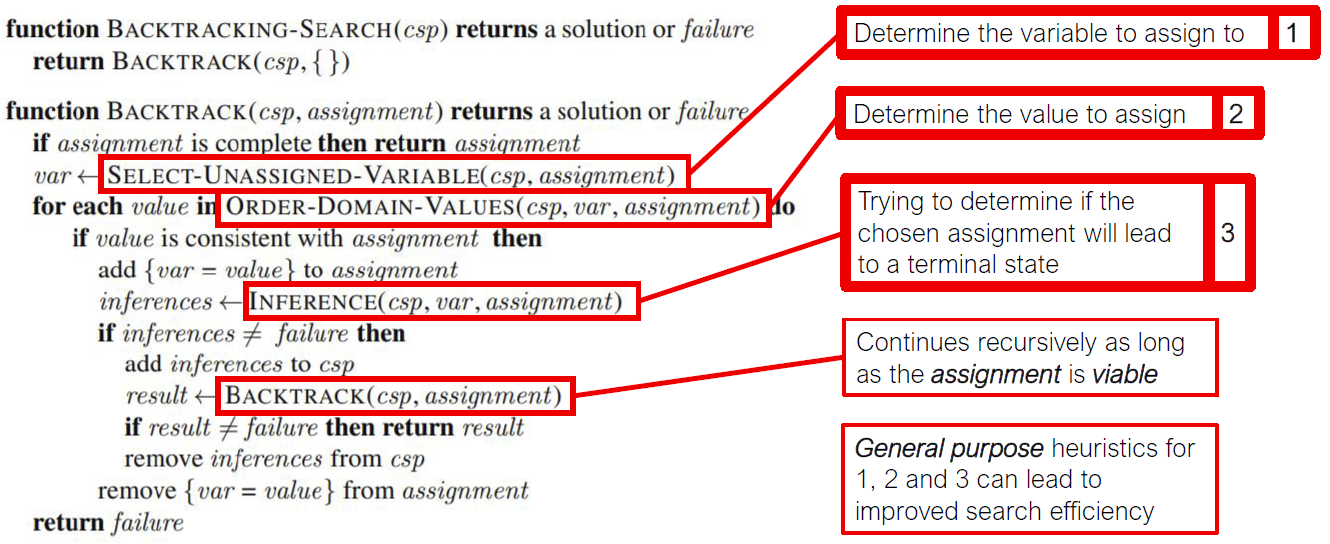
\includegraphics[width=0.7\columnwidth]{backtracking}
	\end{center}
	\subsection{Variable-Order Heuristics}
	\subsubsection{Minimum-Remaining-Values}
	\begin{itemize}
		\item Choose the variable with fewest legal values (most constraint variable)
		\item Idea is to place larger subtrees near the root so that we can eliminate larger subtrees earlier if we find any invalid states
		\item Performs better than static or random ordering
	\end{itemize}
	\subsubsection{Degree Heuristic}
	\begin{itemize}
		\item Tie-breaking mechanism of MRV
		\item Picks variables with most constraints relative to unassigned variables
		\item Idea is that by selecting variable that restricts the most number of other variables, we reduce branching factor
	\end{itemize}
	\subsection{Value Order Heuristic}
	\subsubsection{Least-Constraining-Value Heuristic}
	\begin{itemize}
		\item Choose the value that rules out the fewest choices (most choices)
		\item Idea is that when picking values we want to avoid failures (empty domains) to get to a solution as fast as possible
	\end{itemize}
	\subsection{Strategy in picking Variable vs Values}
	\begin{itemize}
		\item With \textbf{variables}, we want to \textbf{fail fast} since it typically leads to fewer successful assignments to backtrack over
		\item With \textbf{values}, want to \textbf{fail last} since it allows us to have more options and thus have a higher probability of reaching a goal node via DFS
	\end{itemize}
	\subsection{Inference Algorithms}
	\subsubsection{Forward Checking}
	\begin{itemize}
		\item Track remaining legal values for unassigned variables and \textbf{terminate search when any variable has no legal values}
		\item Does not provide early detection for failures
	\end{itemize}
	\subsubsection{Constraint Propagation}
	\begin{itemize}
		\item Inference step to ensure local consistency of ALL variables
		\item After action taken, traverse constraint graph and ensure domain of each variable are both \textbf{node} (unary constraint) and \textbf{arc} (binary constraint) consistent
		\item Node-consistency (unary constraint) done as \textbf{pre-processing}
		\item To maintain Arc Consistency, remove any value from the target variable if it makes a constraint impossible to satisfy
		\item Arcs are directed (\textcolor{red}{binary constraint is 2 arcs})
		\item Arc consistency is ran during backtracking or as a pre-processing step. Detects failure earlier than forward checking
		\item For AC, if we check arc($X_a, X_b$) and propagate to check arc($X_b,X_a$), we don't have to check arc($X_a, X_b$) again!
	\end{itemize}
	\columnbreak
	\subsection{AC-3 Algorithm}
	\begin{center}
		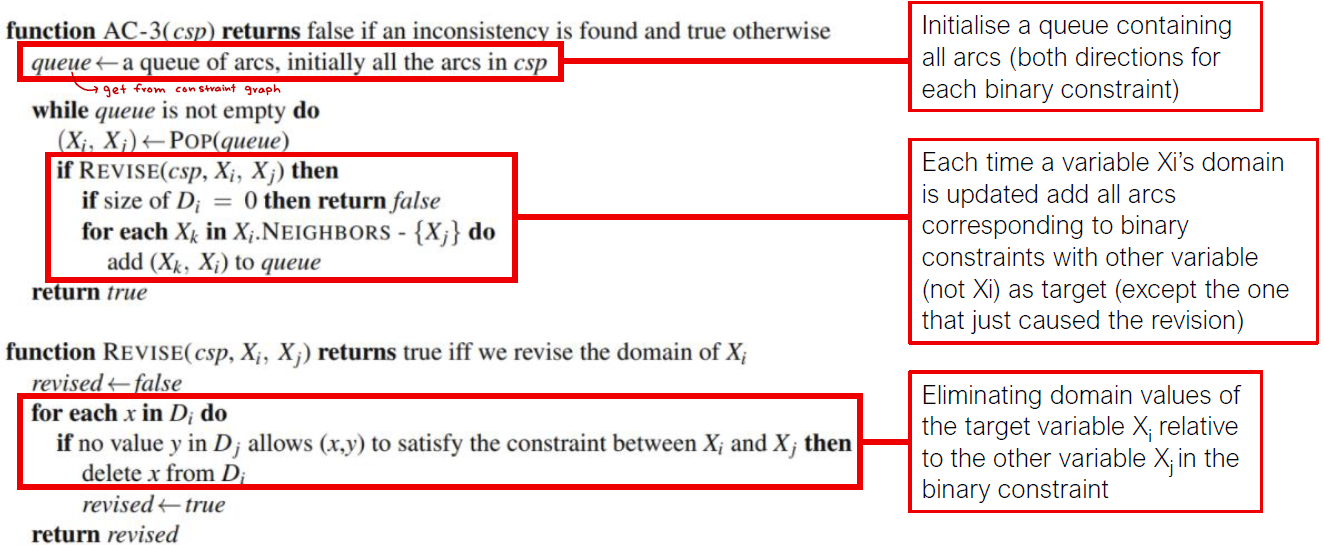
\includegraphics[width=0.7\columnwidth]{ac-3}
	\end{center}
	\subsubsection{Time Complexity of AC-3}
	\begin{itemize}
		\item CSPs have at most 2$\cdot ^nC_2$ or O($n^2$) directed arcs (n variables)
		\item Each arc ($X_i, X_j$) can be inserted at most $d$ times because $X_i$ has at
		most $d$ values to delete (given domain size $d$) - Checking consistency of an arc takes O($d^2$) time
		\item Total time complexity: O($n^2 \times d \times d^2$) = O($n^2d^3$)
	\end{itemize}
	\subsubsection{Maintaining Arc Consistency}
	\begin{itemize}
		\item Run AC as pre-processing step (since it takes a long time to run) to reduce domain sizes and branching factor of search tree
		\item After assignment, use forwards checking as inference (does not ensure arc consistency)
	\end{itemize}
	\section{Adversarial Search}
	\subsection{Games and Search}
	\begin{itemize}
		\item Assumes a zero-sum game (winner gets paid, loser pays) where there are 2 players - MIN and MAX
		\item Simulating a play against a \textbf{utility} maximizing opponent
		\item \textbf{Winning Strategy}: $p_1$ WINS for any strategy $p_2$ takes
		\item \textbf{Non-losing strategy}: $p_1$ WINS or TIES for any strategy $p_2$ takes 
	\end{itemize}
	\subsubsection{Formulating Games}
	\begin{itemize}
		\item \textbf{State} - as per normal search problem
		\item \textbf{TO-MOVE}(state) - returns which player's turn to move given current state
		\item \textbf{ACTION}(state) - Legal moves in state s
		\item \textbf{RESULT}(s, a) - Transition model, returns resultant state after taking action a at state s
		\item \textbf{IS-TERMINAL}(s) - returns whether game is over
		\item \textbf{UTILITY}(s, p) - Gives a numerical value to player p when game ends in a \textbf{terminal state} s
		\begin{itemize}
			\item If assuming zero sum game: UTILITY(MAX, s) + UTILITY(MIN, s) = 0
		\end{itemize}
	\end{itemize}
	\subsection{Minimax Algorithm}
	\begin{center}
		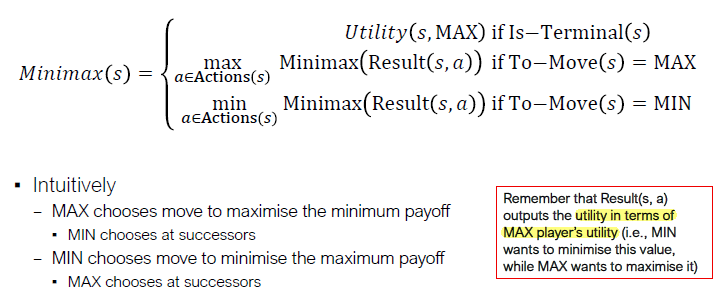
\includegraphics[width=0.6\columnwidth]{minimax}
	\end{center}
	\begin{itemize}
		\item Complete if game tree is finite and optimal (given optimal gameplay)
		\item MAX chooses the move that maximises MAX player utility, MIN chooses move to minimises MAX player utility
		\item Time: O($b^m$), Space: O(bm) - follows DFS
		\item \textbf{Limitation}: In most cases game trees are massive (chess has $10^{123}$ nodes) and we cannot expand entire tree
	\end{itemize}
	\subsection{$\alpha-\beta$ Pruning}
	\begin{itemize}
		\item Idea is to not explore moves that would never be considered
		\item Maintain bounds on values seen thus far while searching
		\begin{itemize}
			\item $\alpha$ bounds MAX's values (highest MAX seen so far)
			\item $\beta$ bounds MIN's values (lowest MIN seen so far)
		\end{itemize}
	\end{itemize}
	\begin{center}
		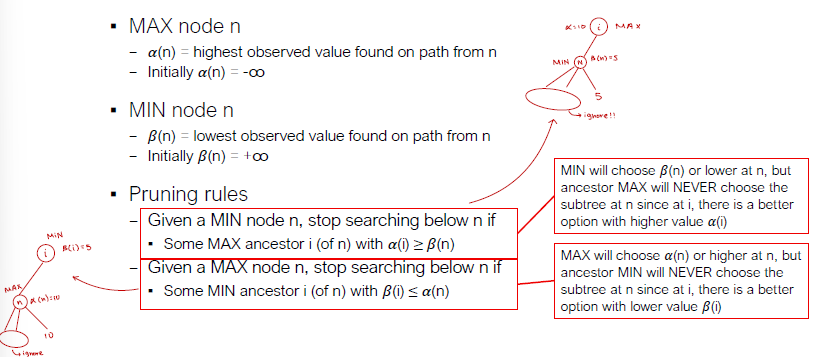
\includegraphics[width=0.7\columnwidth]{a-b-pruning}
	\end{center}
	\begin{itemize}
		\item \textcolor{red}{Ordering matters} for $\alpha$-$\beta$ pruning!!
		\begin{itemize}
			\item "Perfect ordering" will have a time complexity of O($b^{m/2}$)
			\item Random ordering will have complexity of O($b^{3/4m}$)
		\end{itemize}
		\item Faces issues with max depth of tree (traverses to terminal states)
		\item Solved using \textbf{heuristic minimax} - cutoff test (e.g. DLS or IDS) or using evaluation function to estimate expected utility of state
	\end{itemize}
	\columnbreak
	\section{Knowledge Representation}
	\subsection{Recap: Problem Solving Agents}
	\begin{itemize}
		\item Tries to find solution via Search
		\item No real model of what the agent knows
		\begin{itemize}
			\item Each state contains knowledge on state of the whole environment - transition models, actions, implicit knowledge of environment (e.g. path finding has non -ve road lengths)
			\item Atomic representations limiting - e.g. in minesweeper game, environment is partially observable and agent would not know where all mines are
		\end{itemize}
	\end{itemize}
	\subsection{Knowledge-Based/Logical Agents}
	\begin{itemize}
		\item Represent agent domain knowledge using logical formulas
		\item Idea: Make inference on existing information - use old knowledge to infer new knowledge
		\item States similar to CSPs - assignments of values to variables
		\item Agent contains knowledge base and inference engine
		\item Cannot plan entire path to goal since environment is only \textbf{partially observable}
	\end{itemize}
	\subsubsection{Knowledge Base}
	\begin{itemize}
		\item Set of sentences in a formal language (expressive and parsable)
		\item Pre-populate with domain knowledge (rules, general knowledge)
		\item \textbf{Declarative} approach to problem solving
		\begin{itemize}
			\item Tell it what it needs to know - update percepts/state/action
			\item Ask itself what to do = make inferences based on KB on what actions to take
		\end{itemize}
	\end{itemize}
	\begin{center}
		\includegraphics[width=0.7\columnwidth]{kb-agent}
	\end{center}
	\begin{itemize}
		\item Agent must be able to represent states/actions, incorporate new percepts, update internal representation of environment and deduce hidden environment properties and corresponding actions
	\end{itemize}
	\subsection{Entailment}
	\begin{itemize}
		\item $v$ models $\alpha$ if $\alpha$ is true under $v$ (if $v$ makes $\alpha$ true, it models $\alpha$)
		\begin{itemize}
			\item $v$ is one set of value assignments (applied to sentences $\alpha$)
			\item $v$ corresponds to one instance of the environment (known part of a state)
		\end{itemize}
		\item Let $M(\alpha)$ be the set of all models for $\alpha$
		\item Entailment ($\models$) means that one thing follows from the other - e.g. $\alpha \models \beta \equiv M(a)\subseteq M(\beta)$ (can also be understood as $\alpha\rightarrow\beta$)
	\end{itemize}
	\begin{center}
		\includegraphics[width=0.3\columnwidth]{entailment}
	\end{center}
	\subsection{Inferences}
	\subsubsection{Soundness and Completeness}
	\begin{itemize}
		\item KB $\vdash_\mathcal{A} \alpha$  - sentence $\alpha$ is derived/inferred from KB by inference algorithm $\mathcal{A}$
		\item Soundness - $\mathcal{A}$ is sound if KB $\vDash_\mathcal{A}\alpha$ implies KB $\models\alpha$, i.e. $\mathcal{A}$ will not infer nonsense
		\item Completeness -  $\mathcal{A}$ is complete if  KB $\models\alpha$ implies KB $\vDash_\mathcal{A}\alpha$ i.e. $\mathcal{A}$ can infer any sentence that KB entails
	\end{itemize}
	\begin{center}
		\includegraphics[width=0.6\columnwidth]{inf-complete}
	\end{center}
	\subsubsection{Truth Table Enumeration}
	\begin{itemize}
		\item Given a bunch of clauses and $\alpha_1$, KB $\models\alpha_1\leftrightarrow$ whenever KB is true, $\alpha_1$ is also true (if there is a case where KB is true and $\alpha_1$ is false, then KB $\not\models\alpha_1$) 
		\item O($2^n$) time complexity, O(n) space complexity (DFS)
		\item Guaranteed completeness and soundness
	\end{itemize}
	\columnbreak
	\subsection{Proof Methods}
	\begin{itemize}
		\item Model checking (Special case of CSPs where domains are T/F): Proofed using truth table enumeration or resolution
		\item Applying inference rules (i.e. theorem proving), generate new sentence from old and proof using sequential application of inference rules - rules help to deduce valid actions which improves efficiency by ignoring irrelevant proposition
	\end{itemize}
	\subsection{Validity \& Satisfiability}
	\begin{itemize}
		\item Sentence $\alpha$ is valid if it is true for \textbf{ALL} possible truth value assignments (i.e. Tautologies)
		\item Validity is connected to entailment via deduction theorem - (KB$\vDash\alpha$)$\Leftrightarrow$((KB$\Rightarrow\alpha$) is valid) (i.e. entailment = implication)
		\item Sentence is satisfiable if it is true for SOME truth value assignment and unsatisfiable if true for NO truth value assignment (i.e. contradictions)
		\item Satisfiability shown by showing that (KB$\VDash\alpha$)$\Leftrightarrow$((KB$\wedge\neg\alpha$) is unsatifiable)
	\end{itemize}
	\subsection{Inference Algorithm}
	\begin{itemize}
		\item Using inference to grow the knowledge base is similar to a search problem
		\begin{itemize}
			\item \textbf{States}: Versions of KB
			\item \textbf{Actions}: application of inference rules
			\item \textbf{Transition}: update KB with inferred sentence
			\item \textbf{Goal}: KB contains sentence to prove/disprove
		\end{itemize}
		\item Some inference rules
		\begin{itemize}
			\item And-Elimination: $a\wedge b\vDash a$; $a\wedge b \vDash b$
			\item Modus Ponens: $a\wedge(a\Rightarrow b)\vDash b$
			\item Logical Equivalences: $(a\lor b)\vDash \neg(\neg a \wedge \neg b)$
		\end{itemize}
		\item Inference is related to Truth Table Enumeration since it \textbf{goes through all cases} including false ones and \textbf{all inferences are modeled by knowledge base}
	\end{itemize}
	\subsection{Conjunctive Normal Form}
	\begin{itemize}
		\item CNF = Conjunction of disjunctive sentences\\e.g. $(x_1\lor \neg x_2)\wedge (x_2 \lor x_3 \lor \neg x_4)$
		\item Rules for converting to CNF
		\begin{itemize}
			\item $\alpha\Leftrightarrow\beta\equiv(\alpha\Rightarrow\beta)\wedge(\beta\Rightarrow\alpha)$
			\item $\alpha\Rightarrow\beta\equiv\neg\alpha\lor\beta$
			\item $\neg(\alpha\lor\beta)\equiv\neg\alpha\wedge\neg\beta$
			\item $\neg(\alpha\wedge\beta)\equiv\neg\alpha\lor\neg\beta$
			\item $\neg(\neg\alpha)\equiv\alpha$
			\item $\left(\alpha\lor(\beta\wedge\gamma)\right)\equiv(\alpha\lor\beta)\wedge(\alpha\lor\gamma)$
		\item $\alpha \oplus \beta = (\neg\alpha\lor\neg\beta)\land (\alpha\lor\beta)$
		\end{itemize}
	\end{itemize}
	\subsection{Resolution Algorithm}
	\begin{itemize}
		\item Method of simplifying KB to prove entailment of query $\alpha$
		\item Resolution under propositional logic is \textcolor{red}{sound} and \textcolor{red}{complete}
	\end{itemize}
	\begin{center}
		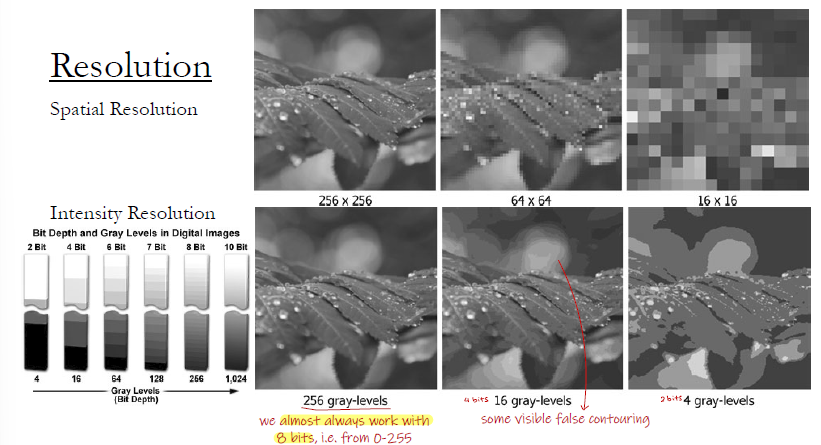
\includegraphics[width=0.7\columnwidth]{resolution}
	\end{center}
	\begin{itemize}
		\item Steps involved:
		\begin{itemize}
			\item Make clause list - copy KB in CNF and add in $\neg\alpha$
			\item Repeatedly resolve 2 clause from clause list and add resolvent to clause list
			\item Keep doing it till empty clause found or no more resolution - empty clause means that we can infer $\alpha$ and if no more resolution available and still not empty clause then $\alpha$ does not hold
			\item Soundness is due to the fact that each resolvent is implied by generating clauses and if $\emptyset$ is found, then (KB$\wedge\neg\alpha$) is unsatisfiable which mean (KB$\wedge\alpha$) must be true
		\end{itemize}
	\end{itemize}
	\section{Baeysian Network}
	\subsection{Dealing with Uncertainty}
	\begin{itemize}
		\item Possible sources of uncertainty:
		\begin{itemize}
			\item Partial observability
			\item Noisy Sensor
			\item Uncertainty in action outcomes
			\item Complexity in modeling and predicting traffic
		\end{itemize}
		\item Logical agent either risk falsehood by saying that an uncertain action WILL get me to a goal or reach a weaker conclusion by saying that it will reach goal given certain constraints
	\end{itemize}
	\columnbreak
	\subsection{Probability Recap}
	\subsubsection{Joint Probability}
	\begin{center}
		\includegraphics[width=0.6\columnwidth]{joint-probability}
	\end{center}
	\subsubsection{Conditional Probability \& Bayes Theorem}
	\begin{itemize}
		\item Pr[A|B]=$\frac{\text{Pr[A}\wedge\text{B}]}{\text{Pr[B]}}$
		\item Pr[A$\wedge$B] = Pr[B|A]$\cdot$Pr[A]
		\item Bayes Rule:  Pr[A|B]=(Pr[B|A]$\cdot$Pr[A])/Pr[B]
		\item If Pr[A$\wedge$ B] = Pr[A]$\cdot$Pr[B], then A and B are independent
		\item Pr[A|B] = Pr[A] if A and B are independent
		\item Pr[A|B] = 1 - Pr[A'|B]
	\end{itemize}
	\subsubsection{Chain Rule}
	\begin{center}
		\includegraphics[width=0.65\columnwidth]{chain-rule}
	\end{center}
	\subsection{Effect of Independence on Joint Probability Table}
	\begin{itemize}
		\item Suppose we have $n$ variable each with domain of size $d$, if the variables are \textbf{not independent}, we will have $d\times d \times \cdots \times d=d^n$ sized table
		\item If the variables are independent, the joint distribution table will be $d+d+\cdots+d=dn$ instead
	\end{itemize}
	\subsection{Conditional Independence in Baeysian Network}
	\begin{itemize}
		\item Want to have as many independence as possible to determine and store less information and also to decrease the number of enumeration needed
		\item Relies heavily on \textbf{conditional independence}, e.g. a person takes 2 ART test, the 2 tests assuming the person has Covid will now be independent - i.e. A, B are independent given knowledge of underlying cause, Pr[A$\wedge$B|S] = Pr[A|S]$\cdot$Pr[B|S]
		\item Full joint distribution table with $n$ boolean variable will have $2^n-1$ entries
		\item With conditional independence a full join distribution table using chain rule becomes: Pr[$T_1\wedge\cdots\wedge T_{n-1}\wedge S$] = Pr[$T_1$|S] $\cdot$ Pr[$T_2$|S] $\cdots$ Pr[$T_{n-1}$|S]$\cdot$ Pr[S], which means we only need to store 2(n-1) + 1 entries
		\item Pr[Cause|Effect] = Pr[Cause] / Pr[Effect]$\cdot$ Pr[Effect|Cause] = $\alpha\cdot$ Pr[Cause] $\cdot$ $\prod_{i=1,...,k}$ Pr[$Effect_i$ | Cause]
	\end{itemize}
	\subsection{Normalization}
	\begin{center}
		\includegraphics[width=0.65\columnwidth]{normalisation}
	\end{center}
	\subsection{Conditional Probability Tables}
	\begin{center}
		\includegraphics[width=0.7\columnwidth]{cpt}
	\end{center}
	\subsection{Baeysian Network}
	\begin{itemize}
		\item Represents joint distributions via a graph
		\begin{itemize}
			\item Vertices are variables and edges from X to Y $\rightarrow$ X directly influences Y (i.e. X causes Y) 
			\item Each node in a bayesian network has a conditional distribution for the node, given its parents.
			\item Max number of edges in Baeysian network = $n(n-1)/2$, complete graph
		\end{itemize}
	\end{itemize}
	\begin{tabular}{c c}
		\includegraphics[width=0.5\linewidth]{baey_net_1}
		\includegraphics[width=0.5\linewidth]{baey_net_2}
	\end{tabular}
	\begin{tabular}{c c}
		\includegraphics[width=0.5\linewidth]{baey_net_3}
		\includegraphics[width=0.5\linewidth]{baey_net_4}
	\end{tabular}
	\begin{center}
		\includegraphics[width=0.7\columnwidth]{baey_net_eg1}
	\end{center}
	\begin{tabular}{c c}
		\includegraphics[width=0.5\linewidth]{baey_net_eg2}
		\includegraphics[width=0.5\linewidth]{baey_net_eg3}
	\end{tabular}
	\subsection{Decision-Theoratic Agents}
	\begin{itemize}
		\item Rationality in the face of uncertainty
		\begin{itemize}
			\item Probability Theory – accounting for uncertainty
			\item Utility Theory – accounting for value (dependent on  agent)
			\item Decision Theory = Probability Theory + Utility Theory
		\end{itemize}
		\item Agent is rational iff it chooses actions that maximise utility
		\item Maximum Expected Utility (MEU) Principle - Pick action with highest utility weighted over probable outcomes
	\end{itemize}
	\begin{center}
		\includegraphics[width=0.7\columnwidth]{dt-agent}
	\end{center}
	\section{Goal Search}
	\begin{itemize}
		\item Path to goal is irrelevant, the goal state itself is the solution.
		\item Advantages: (1) use very little $O(b)$/constant memory, (2) can find reasonable solns in large/infinite continuous state spaces
		\item Useful for \textbf{pure optimization problems}: objective is to find the best state according to an \textbf{objective function}. e.g. Vertex cover, TSP, Boolean Satisfiability Problem (SAT), Timetabling
	\end{itemize}
	\subsection{Hill-climbing Algorithms}
	\subsubsection{Problem Formulation}
	\begin{itemize}
		\item Start with \textbf{complete} state i.e. no partial state (removes build up stage and start checking on 1st iteration)
		\item Each state is a possible solution
	\end{itemize}
	\subsubsection{Steepest Ascent - Greedy}
	\begin{itemize}
		\item Start with random initial state, in each iteration find successor that improves on current state
		\item Requires \textbf{actions} and \textbf{transition} to determine successors
		\item Requires some heuristic to give value to each state e.g. $f(n)=-h(n)$ and find maxima
		\item \textbf{Can be stuck at local maxima} and return non-goal state
		\item Problems arises with \textbf{shoulders/plateau, local maxima or ridge}
	\end{itemize}
	\begin{center}
		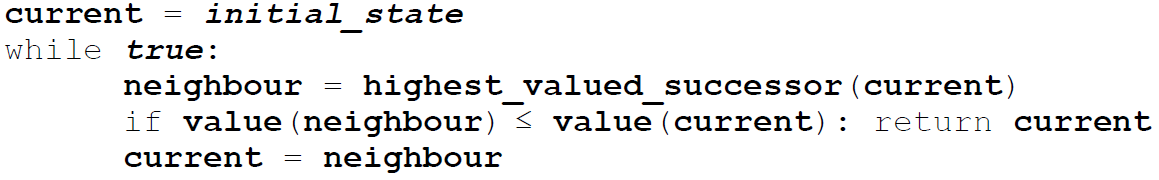
\includegraphics[width=0.75\columnwidth]{hill-climb}
	\end{center}
	\subsubsection{Stochastic Hill Climbing}
	\begin{itemize}
		\item Instead of choosing highest-valued-successor in each step, \textbf{choose randomly among states with better values} instead
		\item Idea is to make the choosing of next state less deterministic to give to algo more chance of finding global maxima
		\item Takes longer but could lead to better solutions
	\end{itemize}
	\subsubsection{First-choice Hill Climbing}
	\begin{itemize}
		\item Handles high branching factor by randomly generating successors until one with better value is found
		\item Possible to achieve $O(1)$ space with this 
	\end{itemize}
	\subsubsection{Sideways Move}
	\begin{itemize}
		\item Replace the $\leq$ sign in steepest ascent with $<$ 
		\item Allows algo to traverse shoulders/plateaus
	\end{itemize}
	\subsubsection{Random-restart}
	\begin{itemize}
		\item Adds outer loop that randomly pick new starting state and keep attempting restarts until solution is found (up to a threshold)
		\item Also allows for sideways move
	\end{itemize}
	\begin{center}
		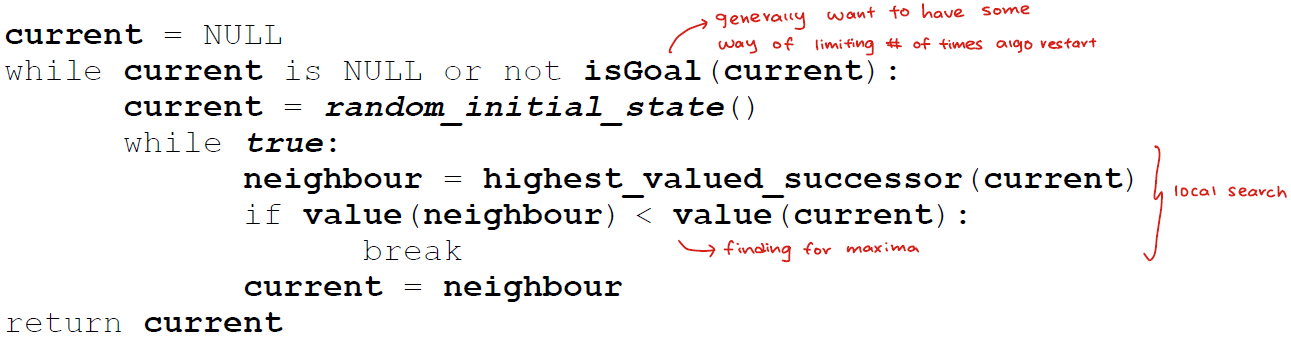
\includegraphics[width=0.8\columnwidth]{random-restart}
	\end{center}
	\subsection{Analysis of Hill Climb}
	\begin{center}
		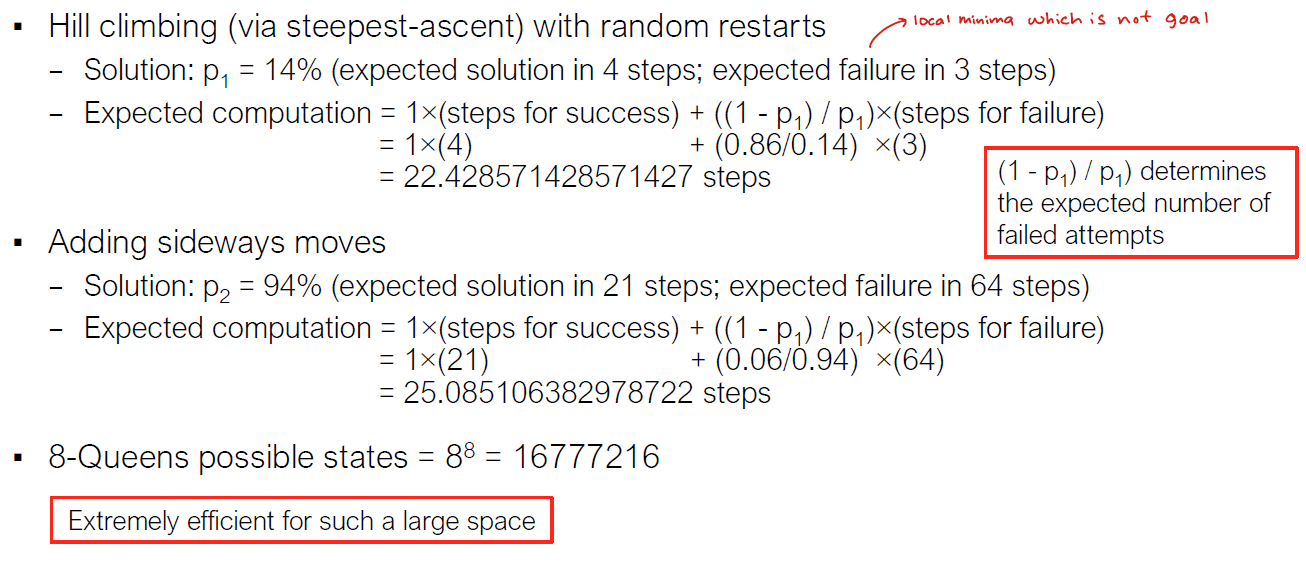
\includegraphics[width=0.9\columnwidth]{hill-climb-analysis}
	\end{center}
	\subsection{Local Beam Search}
	\begin{itemize}
		\item Stores $k$ states instead of 1
		\item Algo begins with $k$ random restarts which generates successors for all $k$ states
		\item Next iteration will repeat the above step with best $k$ among ALL generated successors found (unless goal is found)
		\item Better than $k$ parallel random restarts, Since best $k$ among ALL successors taken (not best from each set of successors, $k$ times)
		\item Also has a stochastic variant to increase probability of escaping from local maxima
	\end{itemize}
	\section{Uninformed Search Summary}
		\textbf{Uninformed Search Strategies}
		
		\begin{tabular}{l|l|l|l|l|l}
			\textbf{Property} & \textbf{BFS} & \textbf{UCS}                                             & \textbf{DFS} & \textbf{DLS} & \textbf{IDS} \\ \hline
			\textbf{Complete} & Yes*         & Yes**                                                    & No***        & No           & Yes*         \\
			\textbf{Optimal}  & No*          & Yes                                                      & No           & No           & No*          \\
			\textbf{Time}     & $O(b^d)$    & $O(b^{1+\left\lfloor\frac{C^*}{\epsilon}\right\rfloor})$ & $O(b^m)$     & $O(b^l)$     & $O(b^d)$     \\
			\textbf{Space}    & $O(b^d)$     & $O(b^{1+\left\lfloor\frac{C^*}{\epsilon}\right\rfloor})$ & $O(bm)$      & $O(bl)$      & $O(bd)$      \\
		\end{tabular}
		
		*: BFS, IDS -- complete if $b$/state space is finite or if there is a solution, optimal if step costs are identical
		
		**: UCS is complete if $b$ is finite and action cost $> \epsilon > 0$
		
		***: DFS is complete only on finite depth \& branching factor graphs
		
		$C^*$ is the optimal cost
	\section{Graph Search Versions}
		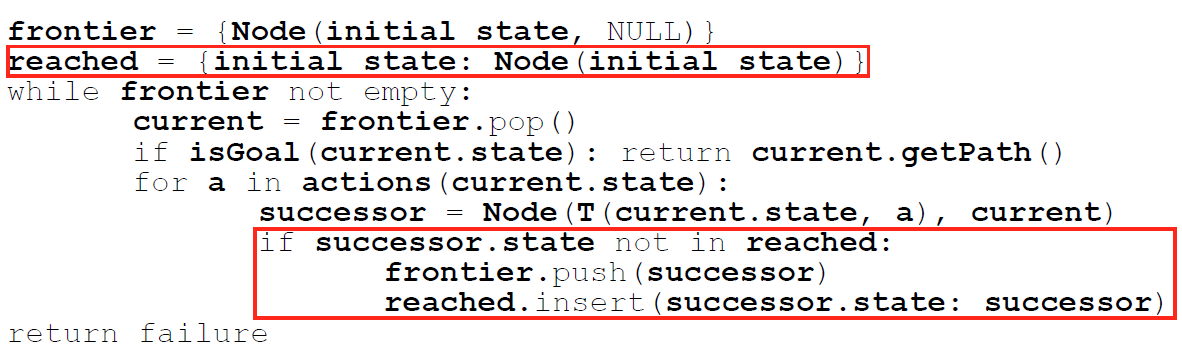
\includegraphics[width=0.8\linewidth]{graph_v1}
		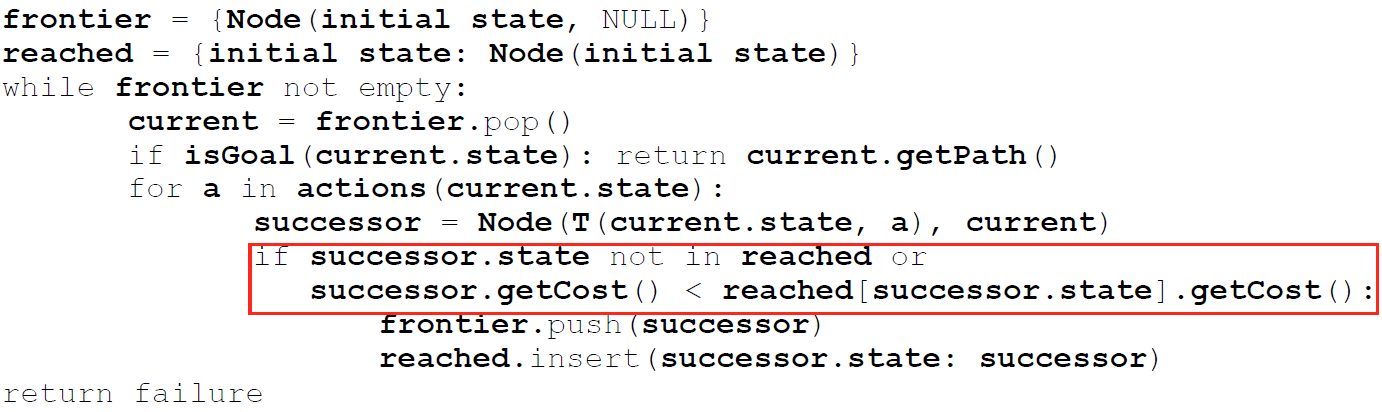
\includegraphics[width=0.8\linewidth]{graph_v2}
		
		Graph search V1 ensures nodes are not revisited which \textcolor{red}{could omit optimal paths}
		
		Graph search V2 solves that by allowing revisits provided cost is lower
		
		Graph search V3 inserts into visited when popped
	\columnbreak
	\section{Heuristics}
	  \begin{itemize}
		\item \textbf{Admissible Heuristic} never overestimates the cost to reach the goal: $\forall n, h(n) \leq h^*(n)$ where $h^*(n) = $ true cost
		\begin{itemize}
			\item Consequence: all paths with actual costs less than $P$ must be searched
		\end{itemize}
		\item \textbf{Consistent Heuristic}: $h(n) \leq c(n, n') + h(n')$, will make $f(n)$ monotonically increasing along a path
		\item \textcolor{red}{Consistency $\implies$ Admissibility}
		\item $h(n)$ is \textbf{admissible}:
		\begin{itemize}
			\item Optimal under \textbf{Tree Search} and \textbf{Graph Search V2}
			\item Non-optimal under \textbf{Graph Search V1}
		\end{itemize}
		\item $h(n)$ is \textbf{consistent}: 
		\begin{itemize}
			\item Optimal under \textbf{Tree Search}, \textbf{Graph Search V2 and V3} (insert into visited when popped)
			\item Non-optimal under \textbf{Graph Search V1}
		\end{itemize}
		\item \textbf{Complete} if $b$ \& $m$ finite OR has a solution and all action cost $> \epsilon > 0$, \textbf{Optimal}, \textbf{Time} $O^{h^*(s_0) - h(s_0)}$ where $h^*(s_0)$ is the actual cost of getting from root to goal, \textbf{Space} $O(b^m)$
		\item \textbf{Dominant heuristic}: if $\forall n, h_2(n) \geq h_1(n)$ then $h_2$ \textbf{dominates} $h_1$
		\item More dominant heuristics incur lower search cost
		\end{itemize}
	\section{Environment Properties}
	\begin{itemize}
		\item \textbf{Fully observable} vs \textbf{Partially observable}: Partially observable agent does not have access to all information (e.g. fully observable maze VS slowly expanding maze based on actions taken). Requires dealing with \textbf{uncertainty} i.e. backtracking algos 
		\item \textbf{Deterministic} vs \textbf{Stochastic}: if the next state of the env is completely determined by the current state and the action executed \textbf{VS} otherwise. (A fully observable environment that has randomness with action is stochastic) (e.g. Sudoku VS Poker)
		\item \textbf{Episodic} vs \textbf{Sequential}: actions only impact current state \textbf{VS} action impact future decisions
		\item \textbf{Discrete} vs \textbf{Continuous}: in terms of state of env, time, percepts and actions (tend to discretize continuous environments)
		\item \textbf{Single agent} vs \textbf{Multi-agent}: whether there are any other agent in the environment whose actions directly influence the performance of this agent, multi-agent further divided into \textbf{competitive} and \textbf{cooperative}
		\item \textbf{Static} vs \textbf{Dynamic}: if the environment is unchanged while an agent is deliberating \textbf{VS} otherwise
	\end{itemize}
	\section{Miscellaneous}
	\subsection{Wumpus World Example}
	\begin{center}
		\includegraphics[width=0.7\columnwidth]{wumpus_world}
	\end{center}
	\subsection{Logical Equivalences}
	\begin{center}
		\includegraphics[width=0.9\columnwidth]{prop_logic}
	\end{center}
%	\begin{itemize}
%		\item Commutative Law: \begin{itemize}
%			\item $p\wedge q\equiv q \wedge p$
%			\item $p \lor q\equiv q \lor p$
%		\end{itemize}
%		\item Associative law:
%		\begin{itemize}
%			\item $(p\wedge q)\wedge r\equiv p \wedge (q\wedge r)$
%			\item $(p\lor q)\lor r\equiv p \lor (q\lor r)$
%		\end{itemize} 
%		\item Distributive law:
%		\begin{itemize}
%			\item $p\wedge(q\lor r)\equiv (p\wedge q)\lor (q\wedge r)$
%			\item $p\lor(q\wedge r)\equiv (p\lor q)\wedge (q\lor r)$
%		\end{itemize}
%		\item Identity Law:
%		\begin{itemize}
%			\item $p\wedge t\equiv p$
%			\item $p\lor c\equiv p$
%		\end{itemize}
%		\item Negation law:
%		\begin{itemize}
%			\item $p\lor \neg p\equiv t$
%			\item $p\wedge \neg p \equiv c$
%		\end{itemize}
%		\item Double Negative Law:
%		\begin{itemize}
%			\item $\neg(\neg p)\equiv p$
%		\end{itemize} 
%		\item Idempotent Law:
%		\begin{itemize}
%			\item $p\wedge p \equiv p$
%			\item $p\lor p \equiv p$
%		\end{itemize} 
%		\item Universal Bound Law:
%		\begin{itemize}
%			\item $p\lor t\equiv t$
%			\item $p \wedge c \equiv c$
%		\end{itemize}
%		\item De Morgan's Law
%		\begin{itemize}
%			\item $\neg(p\wedge q)\equiv \neg p \lor \neg q$
%			\item $\neg(p\lor q)\equiv \neg p \wedge \neg q$
%		\end{itemize}
%		\item Absorption Law:
%		\begin{itemize}
%			\item $p\lor (p\wedge q) \equiv p$
%			\item $p\wedge (p\lor q)\equiv p$
%		\end{itemize}
%	\end{itemize}
	\end{multicols*}
\end{document}
